\section{Design and Implementation}
\label{chp:Design}
According to the working principle of ConAir, there are three main challenges of the design of ConAir.
\begin{itemize}
\item
How to decide the failing point of the program
\item
How to find the idempotent region of the thread
\item
How to realize roll back step
\end{itemize}
\subsection{Identify Failure Sites}
ConAir discusses some types of common errors, including the assertion failures,
wrong output, segmentation fault and deadlock. Most concurrency bugs happen in
the former types. For the assertion failures, the tool will identify the
invocation of \_\_assert\_fail(), if it happens, it means assertion error
happens. For the wrong output error, it is very hard for the tool to detect it
because it does not know what the correct output should be. If user can add
assertion in the program to tell the tool what the correct output should be.
Then the tool can identify the failure site as mentioned. For the segmentation
faults, ConAir identifies every dereference of a heap/ global pointer variable
as a  potential segmentation fault failure site. For the deadlock, ConAir
changes every every pthread\_mutex\_lock into pthread\_mutex\_timelock. If it
timeouts, ConAir detects a deadlock problem in the thread.

\begin{figure*}[htbp]
\center
\begin{tabular}[c]{cccc}
\begin{minipage}{0.23\textwidth}
\begin{lstlisting}[language=C]
//assert(e)

  if(e){
  }else{
Failure:

  __assert_fail(...)

  }
\end{lstlisting}
\caption{Assertion Failures}
\end{minipage}
&\begin{minipage}{0.23\textwidth}\begin{lstlisting}[language=C]
//printf("..",e,..);

  if(Assert(e)){
  }else{
Failure:
//developers specify
//Assert(...)
  }
  printf("..",e,..);

\end{lstlisting}
\caption{Wrong Outputs}
\end{minipage}
&\begin{minipage}{0.23\textwidth}\begin{lstlisting}[language=C]
//tmp=*G_ptr;
  l_ptr=G_ptr;
  if(l_ptr>LowerBound){
  }else{
Failure:


  }
  temp=*l_ptr;

\end{lstlisting}
\caption{Segmentation Faults}
\end{minipage}
&\begin{minipage}{0.23\textwidth}\begin{lstlisting}[language=C]
//pthread_mutex_lock(..);
  int ret = pthread_mutex_timedlock(..);
  if (ret!=TIMEOUT){
  }else{
Failure:


  }
\end{lstlisting}
\caption{Deadlock Failures}
\end{minipage}
\end{tabular}
\end{figure*}
%\begin{figure*}[htbp]
%  \begin{center}
%    \begin{tabular}{cccc}
%      \subfigure[Assertion Failures]{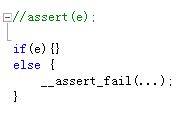
\includegraphics[width=0.24\linewidth]{figs/assertion.png}}&
%      \hspace{-7mm} \subfigure[Wrong Output Failures]{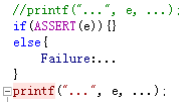
\includegraphics[width=0.24\linewidth]{figs/wrong_output.png}} &
%      \hspace{-7mm} \subfigure[Segmentation Faults]{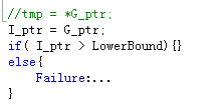
\includegraphics[width=0.24\linewidth]{figs/segmentation_fault.png}}&
%      \hspace{-7mm} \subfigure[Deadlock Failures]{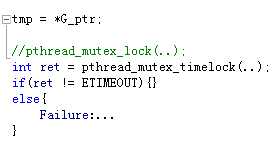
\includegraphics[width=0.24\linewidth]{figs/deadlock_failure.png}} \\
%    \end{tabular}
%  \end{center}
%  \caption{Failure sites for different types of failures}
%  \vspace{-0.5cm}
%\end{figure*}

\subsection{Identify Idempotent Region}
It is very hard to defect failure sites in source code because it is written by users directly without a uniform type. So ConAir chooses to analyze the code in bitcode level. It uses LLVM to transform source code into bitcode. According the rules mentioned in Chapter ~\ref{sbii}, in bitcode level, there still exists rules:\\
\textbf{Idempotency-destroying} with LLVM bitcode:\\
(1)Writes to global or heap variables;
(2)Writes to local variables that are not allocated in virtual registers (static single assignment);
(3)Function-call instructions;
Eliminate codes which are against idempotency, idempotent region in bitcode level can be found.
\subsection{Realize Roll Back Step}
\begin{figure}
  \begin{center}
    \begin{tabular}{cc}
      \subfigure[\label{fig:roll:1}The original
      code]{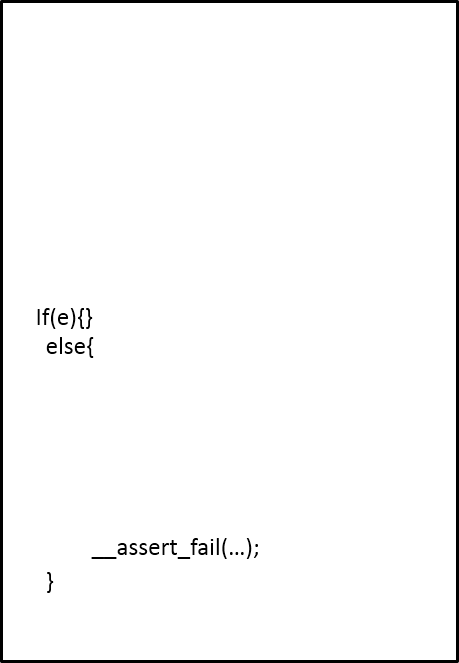
\includegraphics[height=60mm,width=42mm]{figs/rollback_1.png}}&
      \hspace{-7mm}\subfigure[\label{fig:roll:2}The code with roll back]{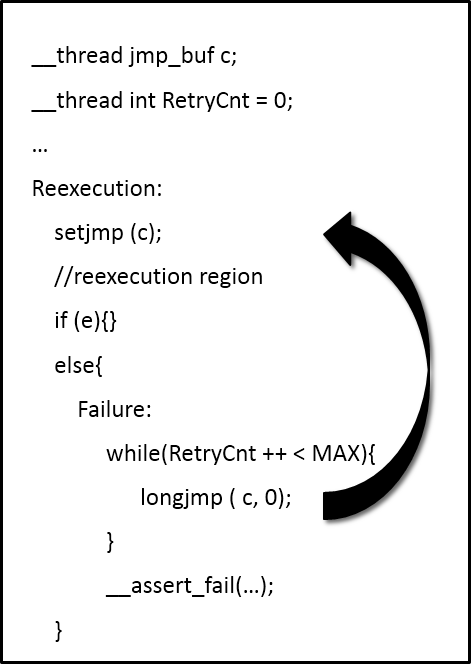
\includegraphics[height=60mm,width=42mm]{figs/rollback_2.png}} \\
    \end{tabular}
  \end{center}
  \vspace{-0.5cm}
  \caption{\label{fig:roll}ConAir code transformation for assert}
\end{figure}
%\begin{figure}
%\begin{minipage}[t]{0.48\linewidth}
%\centering
%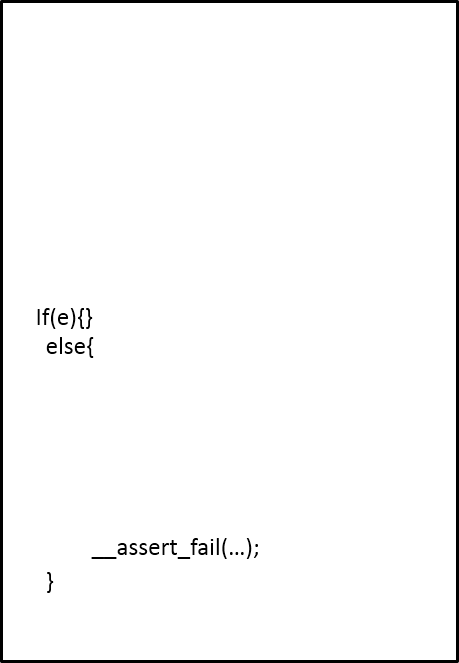
\includegraphics[width=\textwidth]{figs/rollback_1.png}
%\caption{The Origin Code}
%\label {OC}
%\end{minipage}%
%\begin{minipage}[t]{0.48\linewidth}
%\centering
%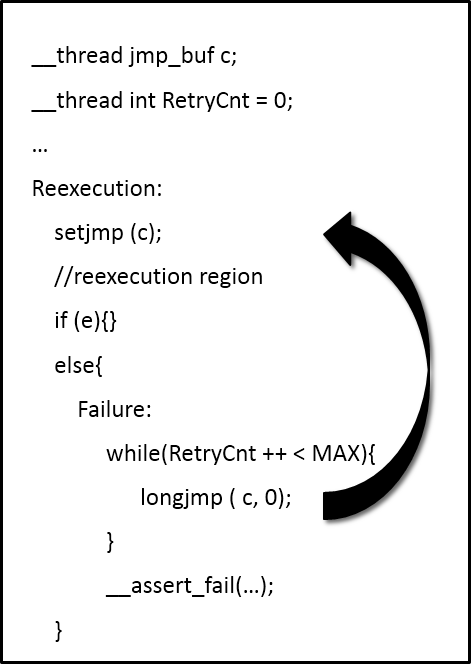
\includegraphics[width=\textwidth]{figs/rollback_2.png}
%\caption{The Code with Roll Back}
%\label{After OC}
%\end{minipage}
%\end{figure}
The roll back is realized by two functions in C++, named setjmp() and longjmp().
longjmp() is inserted in the line before failing site and setjmp() is inserted
in the beginning of idempotent region. When program goes to longjmp(), it will
jump to setjmp() instead of carrying on. Then the roll back is realized.Figure
\ref{fig:roll:2} is the code which ConAir execute and the Figure
\ref{fig:roll:1} is the origin one.

